\section{Laplace Theorie}
Die Laplace-Analysis ist die Weitereentwicklung der Fourier-Analysis $s = \rho + j\omega$. Sie transformiert ein Zeit-basiertes Signal in die Spektralebenen, auch S-Ebene gennant.
\begin{align*}
	F(s) &= \int_{0}^{\infty}f(t)e^{-st}dt \\
	f(t) &= \frac{1}{2\pi j}\int_{\rho_0 - j\infty}^{\rho_0 + j \infty}F(s)e^{st}ds
\end{align*}

\subsection{Eigenschaften}
Siehe Laplace-Tabelle

\subsection{DGL}
\textbf{Beispiel} $\ddot{u}(t) + \dot{u}(t) + u(t) = \sigma(t)\sin(2t)$ mit Anfang $u(0) = 0$ und $\dot{u}(0) = 0$
\[\dot{u}(t) \transform sU(s) - u(0+) \text{ und } \ddot{u}(t) \transform s^2U(s) - sU(0+) - \dot{u}(0+)\]
Dabei werden die Anfangswerte mit Limes identifizert zB: $u(0+) = \lim\limits_{t\rightarrow0+}u(t) = u(0) = 0$.
\[ \sigma(t)\sin(2t) = \frac{2}{s^2 + 2^2} \]
Nun wird die DGL in den Bildbereich transformiert.
\begin{align*}
	s^2U(s) + sU(s) + U(s) &= \frac{2}{s^2 + 2^2} \\
	U(s) &= \frac{2}{(s^2 + 4)(s^2 + s + 1)}
\end{align*}
Mittels PBZ kann dies wieder in den Zeitbereich transformiert werden.
\begin{align*}
	\frac{2}{(s^2 + 4)(s^2 + s + 1)} = \frac{as +b}{s^2 + 4}+\frac{cs + d}{s^2 + s + 1} \quad | \cdot HN \\
	2 = (a + c)s^3 + (a+b+d)s^2 + (a+b+4c)s + b + 4d
\end{align*}
Daraus lässt sich das LGS herleiten und die Parameter mit Koeffizientenvergleich bestimmen.
\[
\begin{matrix}
	a &  &   & + & c  &    &     & = 0 \\
	a &+ & b & + &    & +  & d   &= 0 \\
	a &+ & b & + & 4c &    &     & = 0 \\
	  &  & b &   &    & +  & 4d  & = 2\\
\end{matrix} \qquad\xRightarrow[]{}\qquad
\begin{matrix}
	a &= \frac{-2}{13} \\
	b &=\frac{-6}{13} \\
	c &=\frac{2}{13} \\
	d &= \frac{8}{13}\\
\end{matrix}
\]
Zurück in den Zeitbereich transformieren mittels Umformungen (hier Quadratische Ergänzung $s^2 + s +1 = (s+\frac{1}{2})^2 + \frac{3}{4}$) und Laplace-Tabelle.
\begin{align*}
	U(s) =& -\frac{2}{13}\cdot\overbrace{\frac{s}{s^2 +2^2}}^{\cos(2t)} -\frac{2}{13}\cdot\frac{3}{2}\cdot\overbrace{\frac{2}{s^2 + 2^2}}^{\sin(2t)} \\
	     & + \frac{2}{13}\cdot\underbrace{\frac{s + \frac{1}{2}}{(s+\frac{1}{2})^2 + \frac{3}{4}}}_{\cos\left(\frac{\sqrt{3}}{2}t\right)e^{-\frac{t}{2}}} + \frac{2}{13}\cdot\frac{7\sqrt{3}}{3}\cdot\underbrace{\frac{\frac{\sqrt{3}}{2}}{(s+\frac{1}{2})^2 + \frac{3}{4}}}_{\sin\left(\frac{\sqrt{3}}{2}t\right)e^{-\frac{t}{2}}} \\
\end{align*}
\begin{align*}
	u(t) = \sigma(t)&\left(-\frac{2}{13}\cos(2t) -\frac{3}{13}\sin(2t)\right) \\
	 	   + \sigma(t)&\left( \frac{2}{13}\cos\left(\frac{\sqrt{3}}{2}t\right)e^{-\frac{t}{2}} + \frac{14\sqrt{3}}{39}\sin\left(\frac{\sqrt{3}}{2}t\right)e^{-\frac{t}{2}}\right)
\end{align*}

\subsection{Übertragungsfunktion}\label{ü-funktion}
Die Übertragungsfunktion $G(s)$ ist definiert mit Eingang $x(t) \transform X(s)$ und Ausgang $y(t) \transform Y(s)$ durch 
\[G(s) = \frac{Y(s)}{X(s)} \qquad \text{Frequenzgang}\quad H(\omega) = G(j\omega)\]
Auch bei DGL kann eine Übertragungsfunktion bestimmt werden $\sum_{k=0}^{n}a_k\cdot y^{(k)}(t) = f(t) = \sum_{k=k}^{m}b_k\cdot x^{(k)}(t)$
\[
	G(s) = \frac{q(s)}{p(s)} = \frac{\sum_{k=0}^{m}b_k\cdot s^k}{\sum_{k=0}^{m}a_k\cdot s^k} \xRightarrow[\text{Spez.fall}]{f(t) = x(t)} G(s)=  \frac{1}{\underbrace{\sum_{k=0}^{m}a_k\cdot s^k}_\text{char.polynom}}
\]

\noindent\textbf{Impulsantwort}: $y_{\delta}(t) =  g(t) \transform Y_\delta(s) = G(s)$

\noindent\textbf{Sprungantwort}: $y_{\sigma}(t) = \int_{0}^{t}y_\delta(\tau)d\tau \transform Y_\sigma(s) = \frac{1}{s}G(s)$

\noindent\textbf{Systeme}\\
\begin{center}
	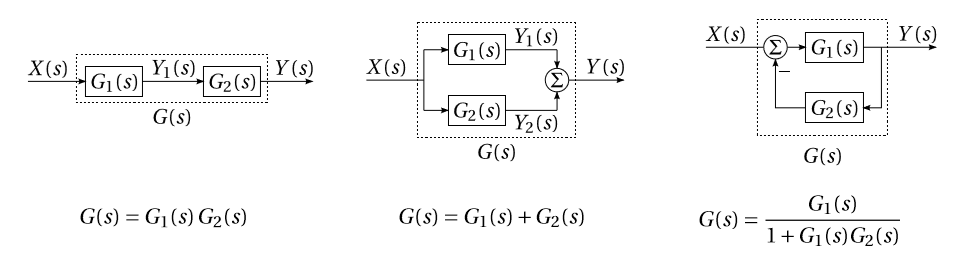
\includegraphics[width=\columnwidth]{Images/systeme}
\end{center}


\subsection{Stabilität}
\textbf{BIBO-Stabilität}\\
BIBO-stabil bedeutet, wenn beschränktes Eingangssignal ein beschränktes Ausgangssignal ergibt.
\[
\int_{-\infty}^{\infty}\left|h(t)\right|dt < \infty
\]

Beispiel: $y(t) = e^tx(t)$ ist instabel, linear und zeitvarient. $y(t)t = \frac{x^4(t)}{1000}$ ist BIBO-stabil, nicht linear und zeitvariant.
\\ ~\\
\textbf{Asymptotische Stabilität}\\
Ein LTI-System ist asymptotisch stabil, wenn seine Impulsantwort asymptotische gegen Null abklingt d.H. $\lim\limits_{t\rightarrow\infty}h(t) = 0$.

\noindent\underline{Instabil}: Wenn mindestens ein Pol in der Rechten s-Halbebene liegt oder wenn ein mehrfach Pol (zB $\frac{1}{(s^2 + 1)^2} \rightarrow \pm j$) auf der j-Achse liegt.\\
\underline{Grenzstabilität}: Wenn kein Pol in der rechten s-Halbebene liegt und kein mehrfach Pol und mindestens ein einfacher Pol auf der j-Achse liegt.\\
\underline{Stabil:} Pol nur in der linken s-Halbebene.\\

\noindent Die Stabilität eines Polynom $P(s) = a_ns^n + a_{n-1}s^{n-1}+a_1s + a_0$ kann auch durch die \textbf{Hurwitz-Kriterium} überprüft werden. 
\underline{stabil}: alle Koeffizienten $a_i > 0$ für $i \in [0;n]$ und die Hurwitz-Determinante $D_i > 0$ für $i\in[1;n]$.

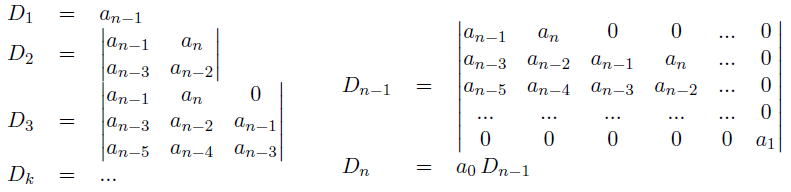
\includegraphics[width=\columnwidth]{Images/hurwitz}

